In this chapter some optimization methods are described and evaluated. Since a deeper discussion would be out of scope only a brief overview is given. Currently almost 80\% of the simulation time is spend on the SOR-Solver for the polarization equation. As a consequence most of the work was spend on the SOR-Solver.
\section{OpenMP}
The complete calculation of the \ac{rhs} for the density and parallel velocities equations can be parallelized without negative consequences. Most gain gives us the parallelization over the z-direction. This is achieved with a simple OpenMP \textit{"for"} worksharing construct as is it is described in \autoref{sec:open-mp-method}. Parallelization in x-direction is only effective for 2D simulations or for very high resolutions. Using the construct on the y-direction is not useful since this loop is always vectorized by the compiler yielding much higher performance. Since the SOR-Solver only works in xy-direction the parallelization in z-direction is effective as well.

\section{Nvidia-CUDA}
To further optimize the SOR-solver and reduce execution time the iteration is moved to the graphics card. This creates some overhead since data has to be moved back and forth to the GPU. Also since there is usually only one GPU available the parallelization in z-direction is not possible anymore. Scaling for different systems is presented later.

\section{Evaluation}
To evaluate performance in a realistic situation it is measured using an actual simulation. A single measurement consists of having the simulation run 1000 iterations and taking the time. Also measured is how much the different steps of each iteration take.\newline
The code is tested on four different systems:
\begin{itemize}
    \item \textbf{\ac{K40C}}: Intel Xeon E3-1225 V2; 16GB RAM;
    \item \textbf{\ac{K40}}: Intel Xeon E3-1225 V2; 16GB RAM; Nvidia K40
    \item \textbf{\ac{GTX}}: 2x Intel Xeon Bronze 3104; 12x 8GB RAM; 7x Nvidia GTX 1080 Ti
    \item \textbf{\ac{TV}}: 2x Intel Xeon Gold 6130; 12x 16GB RAM; 4x Nvidia Titan V
\end{itemize}
Three versions are tested against each other. The first version only runs on the CPU. The second version executes the \ac{SOR}-Solver on the GPU(s). The third version tries to balance the work between GPU and CPU for the \ac{SOR}-Solver. All versions are compiled with \textit{-march=native -O3} and for the different systems the corresponding cuda compute architecture versions.  Four different resolutions (z,x,y) are tested:
\begin{enumerate}
    \item 8x128x128
    \item 8x128x256
    \item 8x256x512
    \item 8x512x1024
\end{enumerate}

\section{Comparison}
\begin{figure}[!hbtp]
    \centering
    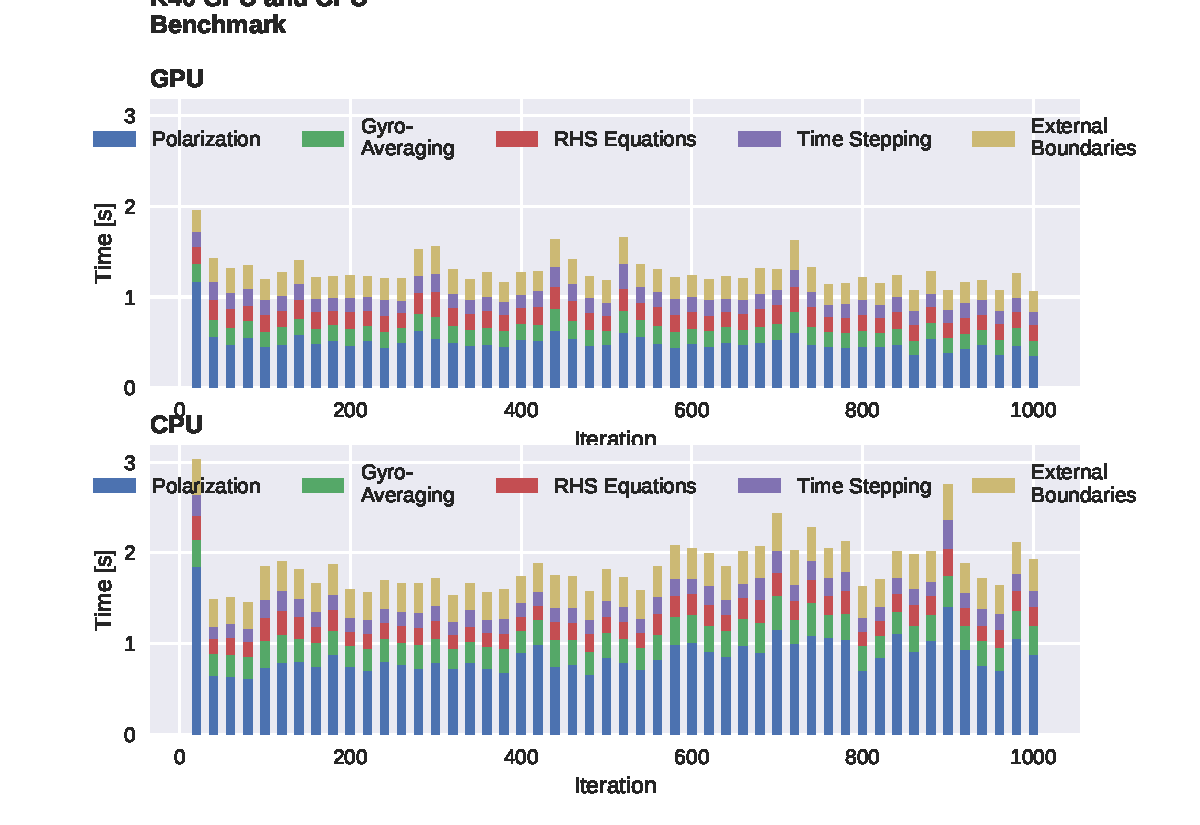
\includegraphics[width=\linewidth]{pdfs/k40CPUvsGPU_full.pdf}
    \caption{Caption}
    \label{fig:my_label}
\end{figure}

\section{Scaling}
\subsection{Scaling on CPU only}
\subsection{Scaling on CPU/GPU systems}
\subsection{Scaling on CPU/GPU sharing}